%%%%%%%%%%%%%%%%%%%%%%%%%%%%%%%%%%%%%%%%%
% Beamer Presentation
% LaTeX Template
% Version 1.0 (10/11/12)
%
% This template has been downloaded from:
% http://www.LaTeXTemplates.com
%
% License:
% CC BY-NC-SA 3.0 (http://creativecommons.org/licenses/by-nc-sa/3.0/)
%
%%%%%%%%%%%%%%%%%%%%%%%%%%%%%%%%%%%%%%%%%

%----------------------------------------------------------------------------------------
%	PACKAGES AND THEMES
%----------------------------------------------------------------------------------------

\documentclass{beamer}

\mode<presentation> {

% The Beamer class comes with a number of default slide themes
% which change the colors and layouts of slides. Below this is a list
% of all the themes, uncomment each in turn to see what they look like.

%\usetheme{default}
%\usetheme{AnnArbor}
%\usetheme{Antibes}
%\usetheme{Bergen}
%\usetheme{Berkeley}
%\usetheme{Berlin}
%\usetheme{Boadilla}
%\usetheme{CambridgeUS}
%\usetheme{Copenhagen}
%\usetheme{Darmstadt}
%\usetheme{Dresden}
%\usetheme{Frankfurt}
%\usetheme{Goettingen}
%\usetheme{Hannover}
%\usetheme{Ilmenau}
%\usetheme{JuanLesPins}
%\usetheme{Luebeck}
\usetheme{Madrid}
%\usetheme{Malmoe}
%\usetheme{Marburg}
%\usetheme{Montpellier}
%\usetheme{PaloAlto}
%\usetheme{Pittsburgh}
%\usetheme{Rochester}
%\usetheme{Singapore}
%\usetheme{Szeged}
%\usetheme{Warsaw}

% As well as themes, the Beamer class has a number of color themes
% for any slide theme. Uncomment each of these in turn to see how it
% changes the colors of your current slide theme.

%\usecolortheme{albatross}
%\usecolortheme{beaver}
%\usecolortheme{beetle}
%\usecolortheme{crane}
%\usecolortheme{dolphin}
%\usecolortheme{dove}
%\usecolortheme{fly}
%\usecolortheme{lily}
%\usecolortheme{orchid}
%\usecolortheme{rose}
%\usecolortheme{seagull}
%\usecolortheme{seahorse}
%\usecolortheme{whale}
%\usecolortheme{wolverine}

%\setbeamertemplate{footline} % To remove the footer line in all slides uncomment this line
%\setbeamertemplate{footline}[page number] % To replace the footer line in all slides with a simple slide count uncomment this line

%\setbeamertemplate{navigation symbols}{} % To remove the navigation symbols from the bottom of all slides uncomment this line
}
\usepackage[
backend=biber,
style=authoryear-icomp,
sortlocale=de_DE,
natbib=true,
url=false, 
doi=true,
eprint=false
]{biblatex}
\addbibresource{bib.bib}
\usepackage{graphicx} % Allows including images
\graphicspath{{Images/}}
\usepackage{caption}
\captionsetup[figure]{font=footnotesize,labelfont=footnotesize}
\usepackage{booktabs} % Allows the use of \toprule, \midrule and \bottomrule in tables

%----------------------------------------------------------------------------------------
%	TITLE PAGE
%----------------------------------------------------------------------------------------

\title[The best privacy defense is a good privacy offense]{The best privacy defense is a good privacy offense: obfuscating a search engine user’s profile} % The short title appears at the bottom of every slide, the full title is only on the title page

\author{Joshua Fenech \& Omar Salbrout} % Your name
\institute[MLDM] % Your institution as it will appear on the bottom of every slide, may be shorthand to save space
{University of Jean Monnet \\ % Your institution for the title page
\medskip
\textit{jfenech22@hotmail.com} % Your email address
}
\date{\today} % Date, can be changed to a custom date

\begin{document}

\begin{frame}
\titlepage % Print the title page as the first slide
\end{frame}

\begin{frame}
\frametitle{Overview} % Table of contents slide, comment this block out to remove it
\tableofcontents % Throughout your presentation, if you choose to use \section{} and \subsection{} commands, these will automatically be printed on this slide as an overview of your presentation
\end{frame}

%----------------------------------------------------------------------------------------
%	PRESENTATION SLIDES
%----------------------------------------------------------------------------------------

%------------------------------------------------
\section{First Section} % Sections can be created in order to organize your presentation into discrete blocks, all sections and subsections are automatically printed in the table of contents as an overview of the talk
%------------------------------------------------

\subsection{Subsection Example} % A subsection can be created just before a set of slides with a common theme to further break down your presentation into chunks


%------------------------------------------------
\section{Introduction}
\subsection{Why we need to protect ourselves}
\begin{frame}
\frametitle{Companies can't be trusted}
\begin{minipage}{0.4\textwidth}
	\vbox to \textheight{
		\vfill
		\centering
		\begin{figure}
		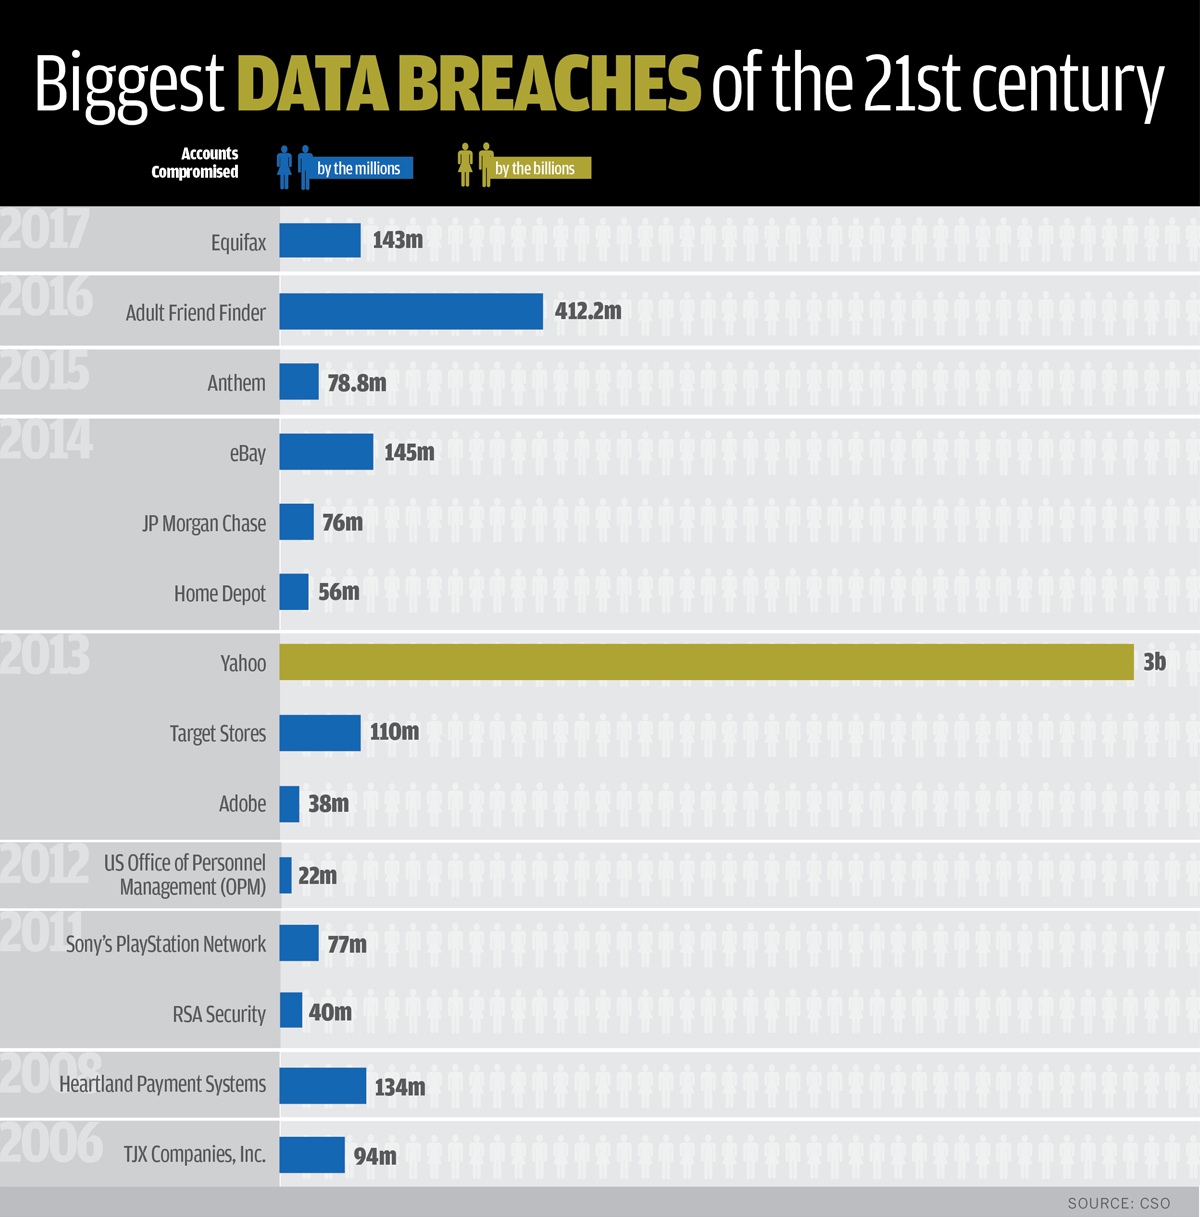
\includegraphics[width=1\textwidth]{biggest-data-breaches.jpg}
		%\caption{www.csoonline.com/article/2130877/data-breach/the-16-biggest-data-breaches-of-the-21st-century.html}
		\end{figure}
		\vfill
	}
\end{minipage}\hfill
\begin{minipage}{0.6\textwidth}
	\vbox to \textheight{
		\begin{itemize}
			\item We trust that companies will protect our data
			\item Data breaches are commonplace today
			\item Unencrypted data is often leaked
			\item There is currently no or little legal requirement to protect data, and therefore represents an additional cost that some companies try to avoid
			\item Can we encrypt our own data before it is submitted to such companies?
		\end{itemize}
		\vfill
	}
\end{minipage}

\end{frame}

%------------------------------------------------

\begin{frame}
\frametitle{Other methods of obfuscation}
\begin{minipage}{0.4\textwidth}
	\vbox to \textheight{
		\vfill
		\centering
		\begin{figure}
			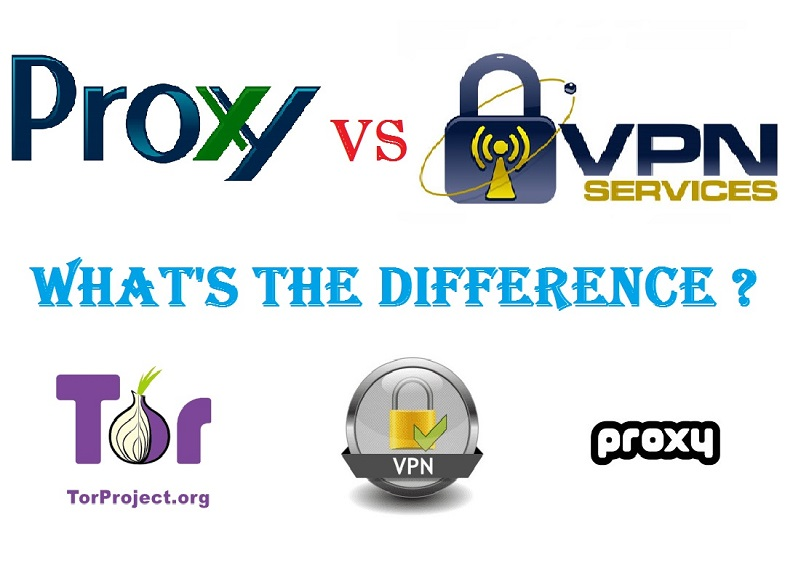
\includegraphics[width=1\textwidth]{torvproxyvvpn.jpg}
			%\caption{www.csoonline.com/article/2130877/data-breach/the-16-biggest-data-breaches-of-the-21st-century.html}
		\end{figure}
		\vfill
	}
\end{minipage}\hfill
\begin{minipage}{0.6\textwidth}
\begin{itemize}
	\item Private browsing - no cookies stored, but... IP still revealed
	\item Proxy servers to hide IP, but... web browser fingerprints still revealed
	\item Ultimately, TOR for maximum anonymity
	\item Problem - lose benefits that personalisation of websearches provides
	\item Can an alternative means of securing privacy without more intensive [change intensive here] methods be found?
\end{itemize}
\end{minipage}
\end{frame}
%------------------------------------------------

\begin{frame}
\frametitle{Structure of Presentation}
\begin{itemize} %NeED TO FIX THIS can do at end
	\item How do search engines know what we want?
	\item Present a new method of obfuscation related to adversarial data mining
	\item Approach is explored in common setting of Internet search engines
	\item A learning method is presented for environments where a user can get feedback from her or his counterpart
\end{itemize}
\end{frame}




%------------------------------------------------
\section{How do search engines know what we want?}
%------------------------------------------------

\begin{frame}
\frametitle{Personalised Advertising}
\begin{minipage}{0.4\textwidth}
	\vbox to \textheight{
		\vfill
		\centering
		\begin{figure}
			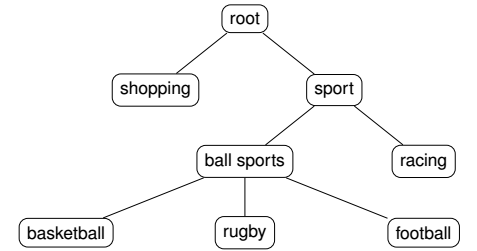
\includegraphics[width=1\textwidth]{search_tree.png}
			%\caption{www.csoonline.com/article/2130877/data-breach/the-16-biggest-data-breaches-of-the-21st-century.html}
		\end{figure}
		\vfill
	}
\end{minipage}\hfill
\begin{minipage}{0.6\textwidth}
	\begin{itemize}
		\item Which ad is displayed depends on:
		\begin{itemize}
			\item[--] The submitted query
			\item[--] The user profile
		\end{itemize}
		\item Ads are assigned to categories
		\item users are assigned to categories
	\end{itemize}
\end{minipage}

\end{frame}

%------------------------------------------------

\begin{frame}

\end{frame}

%------------------------------------------------

\begin{frame}
\end{frame}

%------------------------------------------------

\begin{frame}
\frametitle{Figure}
Uncomment the code on this slide to include your own image from the same directory as the template .TeX file.
%\begin{figure}
%\includegraphics[width=0.8\linewidth]{test}
%\end{figure}
\end{frame}

%------------------------------------------------

\begin{frame}
\end{frame}

%------------------------------------------------

\begin{frame}
\frametitle{References}
\footnotesize{
\begin{thebibliography}{99} % Beamer does not support BibTeX so references must be inserted manually as below
\bibitem[Smith, 2012]{p1} John Smith (2012)
\newblock Title of the publication
\newblock \emph{Journal Name} 12(3), 45 -- 678.
\end{thebibliography}
}
\end{frame}

%------------------------------------------------

\begin{frame}
\Huge{\centerline{The End}}
\end{frame}

%----------------------------------------------------------------------------------------

\end{document} 